\documentclass[12pt]{article}
% \documentclass[twoside,12pt]{book}

\usepackage{fontspec}
\usepackage{titling}
\usepackage[labelfont=bf]{caption}
\usepackage{microtype}
\usepackage{siunitx}
\usepackage{enumitem}
\usepackage{booktabs}
\usepackage{geometry}
\geometry{letterpaper}
% \geometry{letterpaper, textwidth=5.5in, textheight=8.5in, marginparsep=7pt, marginparwidth=.6in}
\usepackage[usenames,dvipsnames]{xcolor}
\usepackage{xunicode}
\defaultfontfeatures{Mapping=tex-text}

\usepackage{pdflscape}
\usepackage{pdfpages}

\graphicspath{{figs/}}

\usepackage[xetex, unicode, bookmarks, colorlinks, breaklinks, pdfusetitle]{hyperref}
\hypersetup{linkcolor=MidnightBlue,citecolor=MidnightBlue,filecolor=black,urlcolor=MidnightBlue} % Link colors

% Linux Libertine Font (default)
\setromanfont{Linux Libertine}
\setsansfont{Linux Biolinum}
% \setmonofont[Scale=0.8]{Iosevka}

% \usepackage{sectsty}
% \allsectionsfont{\sffamily}

\renewcommand{\today}{\ifcase\month\or%
  January\or%
  February\or%
  March\or%
  April\or%
  May\or%
  June\or%
  July\or%
  August\or%
  September\or%
  October\or%
  November\or%
  December\fi~%
\number\year}

\usepackage{lipsum}

\newcommand{\kicad}{Ki\textsc{Cad}}

\begin{document}
\title{\textsc{Fifo} Delay Assembly Information}
\author{Alex Striff}
\date{\today}

\begin{titlingpage} %This starts the title page
    \begin{center}
        \vfill\null%
        \begin{Huge} 
            \thetitle\\
        \end{Huge}
        \vspace{0.5cm}
        \begin{Large}
            \theauthor\\
        \end{Large}
        \vfill\null%
        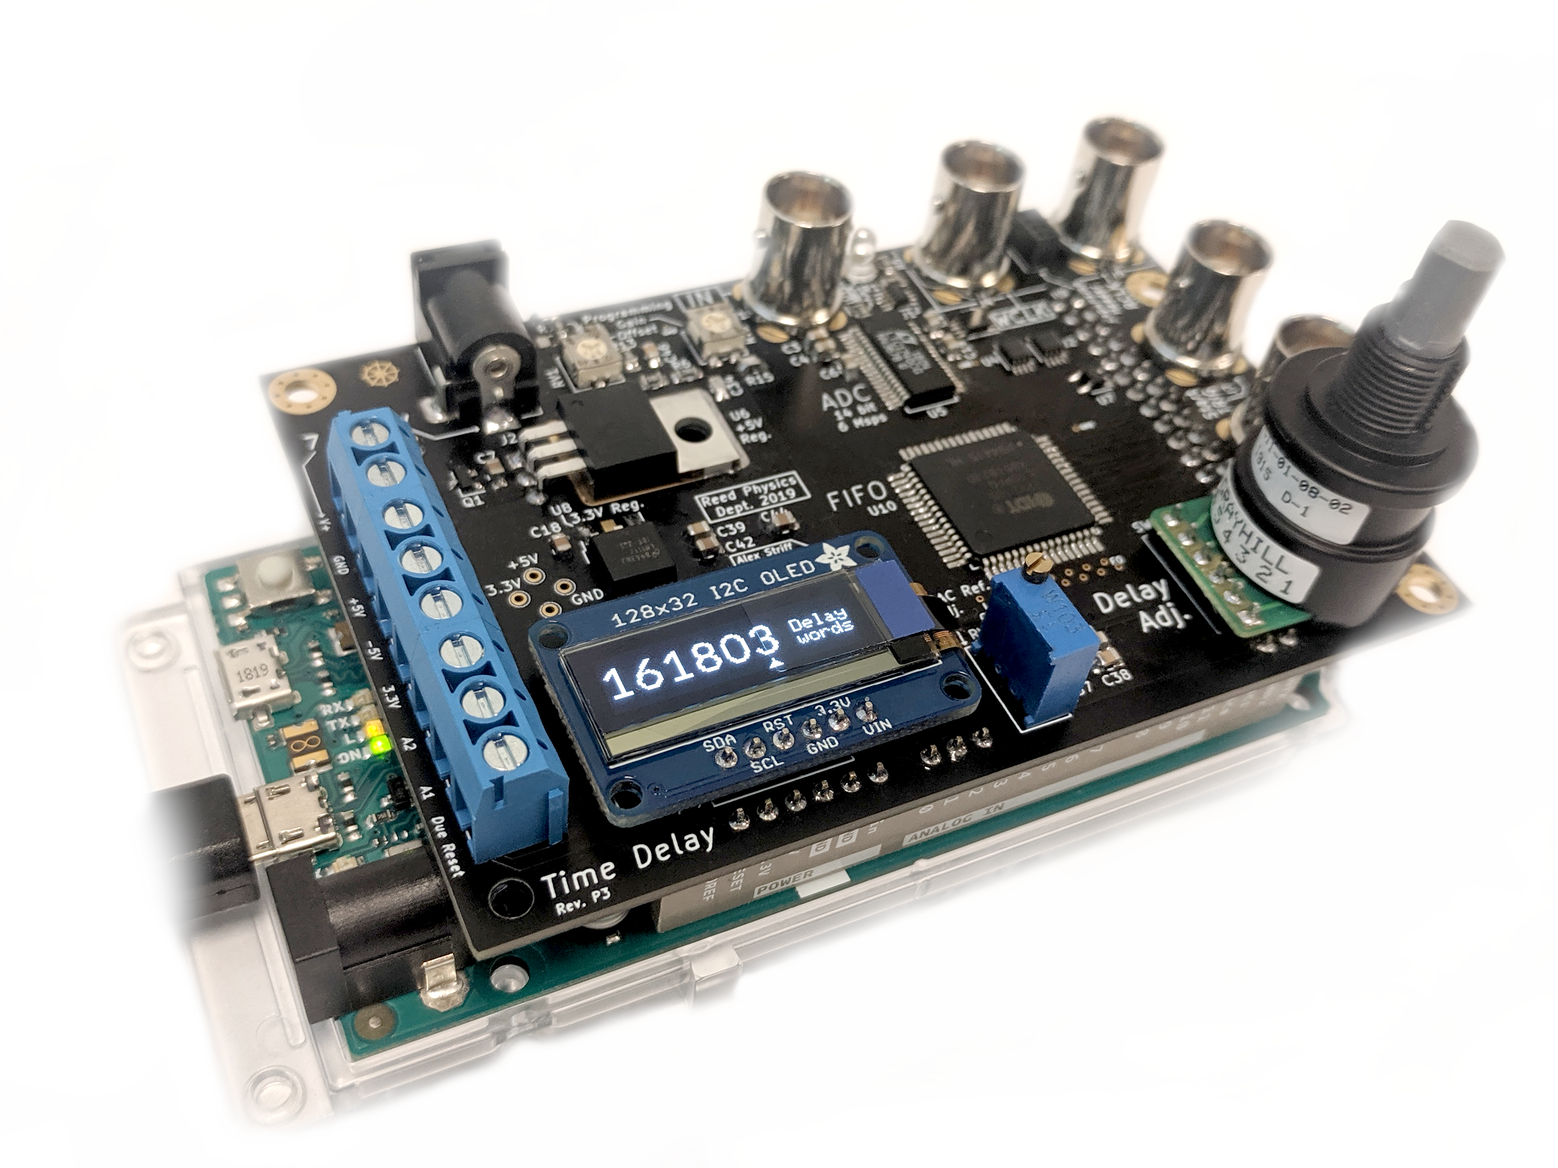
\includegraphics[width=0.625\linewidth]{fifo-p3f-img-small.png}\\
        \vfill\null%
        \begin{large}
        Reed College \\
        Physics Department\\
        \vspace{0.5\baselineskip}
        \thedate%
        \end{large}
        % \vfill\null%
        \tableofcontents%
    \end{center}
\end{titlingpage}

\section{Ordering \textsc{Pcb}s}

Given a complete \href{https://kicad-pcb.org}{\kicad} \textsc{pcb} layout, how
do you order the \textsc{pcb}s?

\subsection{Exporting the \textsc{pcb} files from \kicad}

Circuit board manufacturers expect to receive a \textsc{zip} archive that
contains both the \emph{Gerber} files and \emph{drill} files for a circuit
board. The latest version of the files should exist at
\href{https://github.com/lucasilling/AJP_TimeDelay_Git/tree/master/fifo-p3f/Gerber}{\texttt{/fifo-p3f/Gerber}}
on the \href{https://github.com/lucasilling/AJP_TimeDelay_Git}{GitHub
repository}, but the files may be manually exported from \kicad{} as follows.
With the \textsc{pcb} layout editor open, select \textit{File $\to$ Plot\ldots}
to open the window of Fig.~\ref{fig:gerbers}. Choose an appropriate output
directory and check that all of the correct layers needed for manufacture are
selected, and then select \textit{Generate Drill Files\ldots} to open the window
of Fig.~\ref{fig:mapdrill}. Now set the output directory to be the same as that
for the Gerber files and select the \textit{Generate Drill File} button. You may
also want to generate a map file as a \textsc{pdf} to visually check that the
holes are in reasonable places. Close the drill file window and select
\textit{Plot} in the Gerber file window to generate the Gerber files. You now
should have a directory with several Gerber files for all of the layers and two
drill files (corresponding to plated (\textsc{pth}) and non-plated
(\textsc{npth}) through-holes in the board). Create a \textsc{zip} archive from
the directory of Gerber and drill files. You are now ready to send the files to
a manufacturer.

\begin{figure}
  \centering
  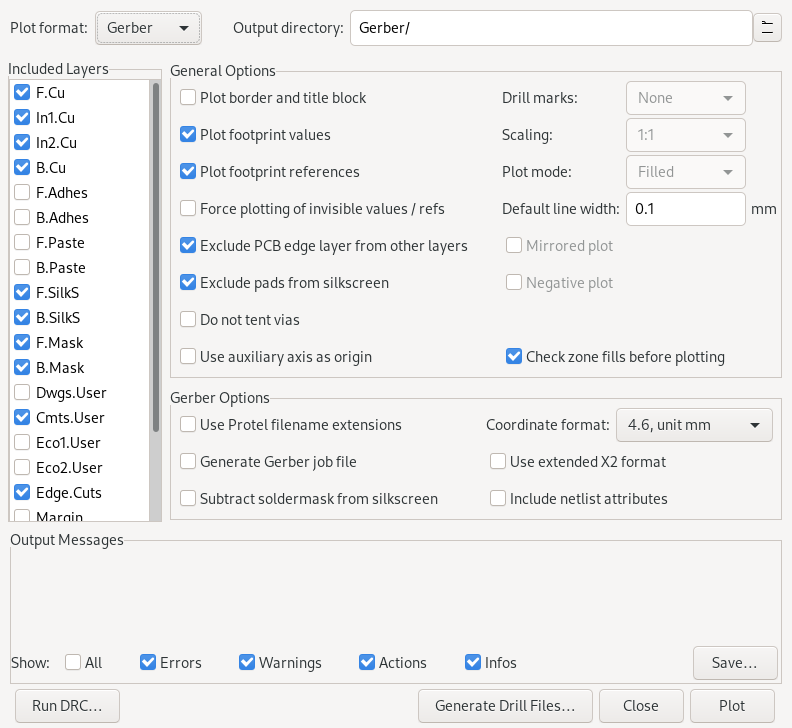
\includegraphics[width=\linewidth]{gerbers}
  \caption{Exporting Gerber files.}\label{fig:gerbers}
\end{figure}

\begin{figure}
  \centering
  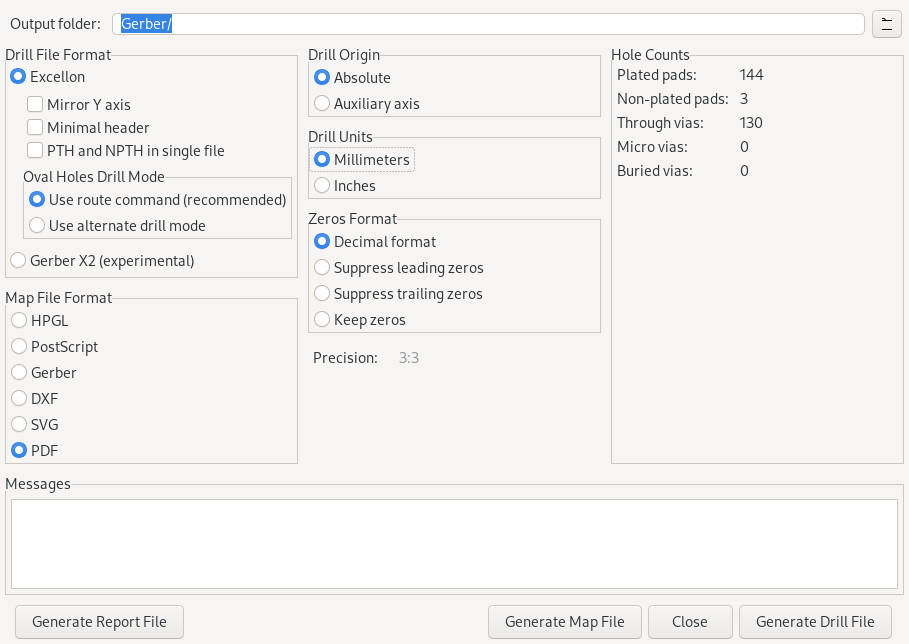
\includegraphics[width=\linewidth]{mapdrill}
  \caption{Exporting drill and map files.}\label{fig:mapdrill}
\end{figure}

\subsection{Sending the files to a manufacturer}

There are many prototyping \textsc{pcb} fabrication houses
available,\footnote{To compare prices for given \textsc{pcb} feature sets, see
\url{pcbshopper.com}.} but the one I have used previously is one of the largest,
cheapest, and most popular: \href{https://jlcpcb.com}{\textsc{JlcPcb}}. It is
straightforward to fill out the forms on these order websites, but be sure to
check that their manufacturing tolerances are below what you
request.\footnote{Our board is easily manufacturable by most fabrication
houses.} The turnaround time for these services varies, but is usually quite
fast: about one week or less with \textsc{dhl} shipping.

\section{Ordering Parts}

A complete
\href{https://github.com/lucasilling/AJP_TimeDelay_Git/blob/master/Digikey_BOM.csv}{bill
of materials} (\textsc{bom}) is given on the
\href{https://github.com/lucasilling/AJP_TimeDelay_Git}{GitHub repository}. To
order the parts, one may simply upload the \textsc{bom} file to
\href{https://www.digikey.com/bom}{Digi-Key} (Fig.~\ref{fig:digikey-bom}). The
relevant entries are reproduced in Table~\ref{tab:bom}. This is useful as a
checklist as you solder parts on to the board.

\begin{figure}[hb]
  \centering
  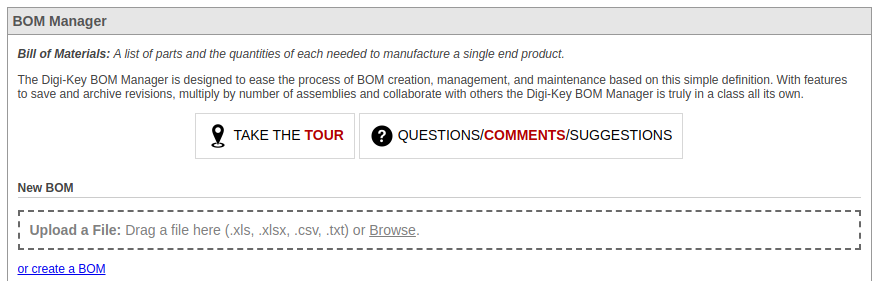
\includegraphics[width=\linewidth]{digikey-bom}
  \caption{The Digi-Key \textsc{bom} manager.}\label{fig:digikey-bom}
\end{figure}

\newgeometry{margin=1in}
\begin{landscape}
\begin{table}[ht]
\caption{Bill of materials. Quantities are sometimes rounded up to a multiple of
ten for price breaks.}\label{tab:bom}
\scriptsize
\begin{tabular}{llllll}
\toprule
Manufacturer Part Number & Digi-Key Part Number     & Customer Reference & Reference Designator                                                      & Quantity & Extended Price \\
\midrule
LM2940CT-5.0/NOPB        & LM2940CT-5.0/NOPB-ND     &                    & U6                                                                        & 1        & 1.53   \\
LM2776DBVR               & 296-43957-1-ND           &                    & U15                                                                       & 1        & 1.02   \\
AD7840ARSZ               & AD7840ARSZ-ND            &                    & U13                                                                       & 1        & 33.39  \\
72V2105L10PFG            & 800-1511-ND              &                    & U10                                                                       & 1        & 131.65 \\
LTC1740CG\#PBF           & LTC1740CG\#PBF-ND        &                    & U5                                                                        & 1        & 41.67  \\
SN74LVC2G157DCTR         & 296-13266-1-ND           &                    & U2                                                                        & 3        & 1.44   \\
931                      & 1528-1169-ND             & 128x32 OLED        & U11                                                                       & 1        & 17.50  \\
TS12A12511DCNR           & 296-27523-1-ND           &                    & U1                                                                        & 1        & 1.45   \\
LM4041DYM3-ADJ-TR        & 576-2573-1-ND            &                    & U14                                                                       & 1        & 0.29   \\
SN74LVC1G04DBVR          & 296-11599-1-ND           &                    & U7                                                                        & 1        & 0.32   \\
SN74LVC1G08DBVR          & 296-11601-1-ND           &                    & U12                                                                       & 1        & 0.26   \\
LM1117IDTX-3.3/NOPB      & LM1117IDTX-3.3/NOPBCT-ND &                    & U8                                                                        & 1        & 1.44   \\
TL082CDR                 & 296-1284-1-ND            &                    & U16                                                                       & 1        & 0.41   \\
A000062                  & 1050-1049-ND             &                    & U9                                                                        & 1        & 37.40  \\
PRPC002SAAN-RC           & S1011EC-02-ND            & Board to board     & U9                                                                        & 2        & 0.16   \\
54102-S08-18             & 609-5600-ND              & Board to board     & U9                                                                        & 1        & 1.45   \\
PRPC003SAAN-RC           & S1011EC-03-ND            & Board to board     & U9                                                                        & 1        & 0.12   \\
PRPC006SAAN-RC           & S1011EC-06-ND            & Board to board     & U9                                                                        & 1        & 0.19   \\
LPPB042CFFN-RC           & S9009E-04-ND             & Board to board     & U9                                                                        & 1        & 1.05   \\
DMP3099L-7               & DMP3099L-7DICT-ND        &                    & Q1                                                                        & 1        & 0.33   \\
151033RS03000            & 732-5013-ND              &                    & D1                                                                        & 1        & 0.17   \\
61C11-01-08-02           & GH6102-ND                &                    & SW1                                                                       & 1        & 25.77  \\
5-1634503-1              & A97581-ND                &                    & J1, J4, J5, J7, J8                                                        & 5        & 11.25  \\
PJ-002A                  & CP-002A-ND               &                    & J2                                                                        & 1        & 0.60   \\
OSTTC082162              & ED2615-ND                &                    & J3                                                                        & 1        & 1.72   \\
TS53YL102MR10            & TS53YL-1.0KCT-ND         &                    & RV1, RV3                                                                  & 2        & 3.74   \\
3296W-1-103LF            & 3296W-103LF-ND           &                    & RV2                                                                       & 1        & 2.41   \\
RC0805FR-0749R9L         & 311-49.9CRCT-ND          &                    & R1, R3, R4, R19                                                           & 4        & 0.40   \\
RC0805FR-0722RL          & 311-22.0CRCT-ND          &                    & R2, R6, R20                                                               & 3        & 0.30   \\
RC0805FR-07220RL         & 311-220CRCT-ND           &                    & R5                                                                        & 1        & 0.10   \\
RC0805FR-075K1L          & 311-5.10KCRCT-ND         &                    & R7, R9, R10, R11, R13, R16, R17, R18                                      & 10       & 0.40   \\
RC0805FR-071K1L          & 311-1.10KCRCT-ND         &                    & R8, R14                                                                   & 2        & 0.20   \\
RC0805FR-073K9L          & 311-3.90KCRCT-ND         &                    & R15                                                                       & 1        & 0.10   \\
RC0805FR-074K3L          & 311-4.30KCRCT-ND         &                    & R12                                                                       & 1        & 0.10   \\
RC0805JR-070RL           & 311-0.0ARCT-ND           & Jumpers            &                                                                           & 10       & 0.35   \\
08055C104KAT2A           & 478-1395-1-ND            & 0u1                & C8, C9, C10, C15, C16, C22, C46,C23, C28, C30, C32, C37, C38              & 20       & 1.66   \\
08053C105KAT2A           & 478-5030-1-ND            & 1u                 & C1, C3, C4, C6, C19, C20, C40, C41,C11, C12, C13, C14, C21, C25, C35, C39 & 20       & 3.52   \\
CL21A106KAYNNNE          & 1276-2891-1-ND           & 10u                & C5, C7, C17, C18, C26, C27, C42, C43, C44, C45,C24, C29, C31, C33         & 20       & 3.80   \\
08055A102JAT2A           & 478-1328-1-ND            & 1n                 & C2,C34, C47                                                               & 10       & 1.26   \\
\bottomrule
\end{tabular}

\end{table}
\end{landscape}
\restoregeometry%

\section{Assembly and Soldering}

Once you have received both parts and boards, you face the task of soldering
them together. If you are unfamiliar with soldering, there are plenty of
resources online, and even surface-mount soldering is easier than it
looks.\footnote{For example,
  \href{https://learn.adafruit.com/adafruit-guide-excellent-soldering/tools}{Adafruit}
covers the basics of through-hole soldering.}
Soldering small \textsc{ic}s with pin pitches of \SI{650}{\um} is simple because
\emph{you} are not doing the fine placement: the surface tension of the solder
is. For that to work, you must be able to control the quantity of solder and
have appropriately prepared surfaces. This is achieved by:
\begin{itemize}
  \item Having good leaded solder with a \emph{small} diameter (less than the
    usual \SI{31}{thou}).
  \item Frequently using a source of flux, such as a flux pen or paste.
\end{itemize}
Mistakes are easily remedied with some solder wick. There is also the
possibility of getting a solder paste stencil with your \textsc{pcb} order and
reflow-soldering the whole board at once.

It is usually a good idea to solder the power supply components first and then
stop to check that the test points give the correct voltages when powered on.
This prevents damage to critical parts like the Arduino or \textsc{fifo} in the
case of an error. Manual continuity checks for densely-packed pins are also a
good idea.

% \begin{landscape}
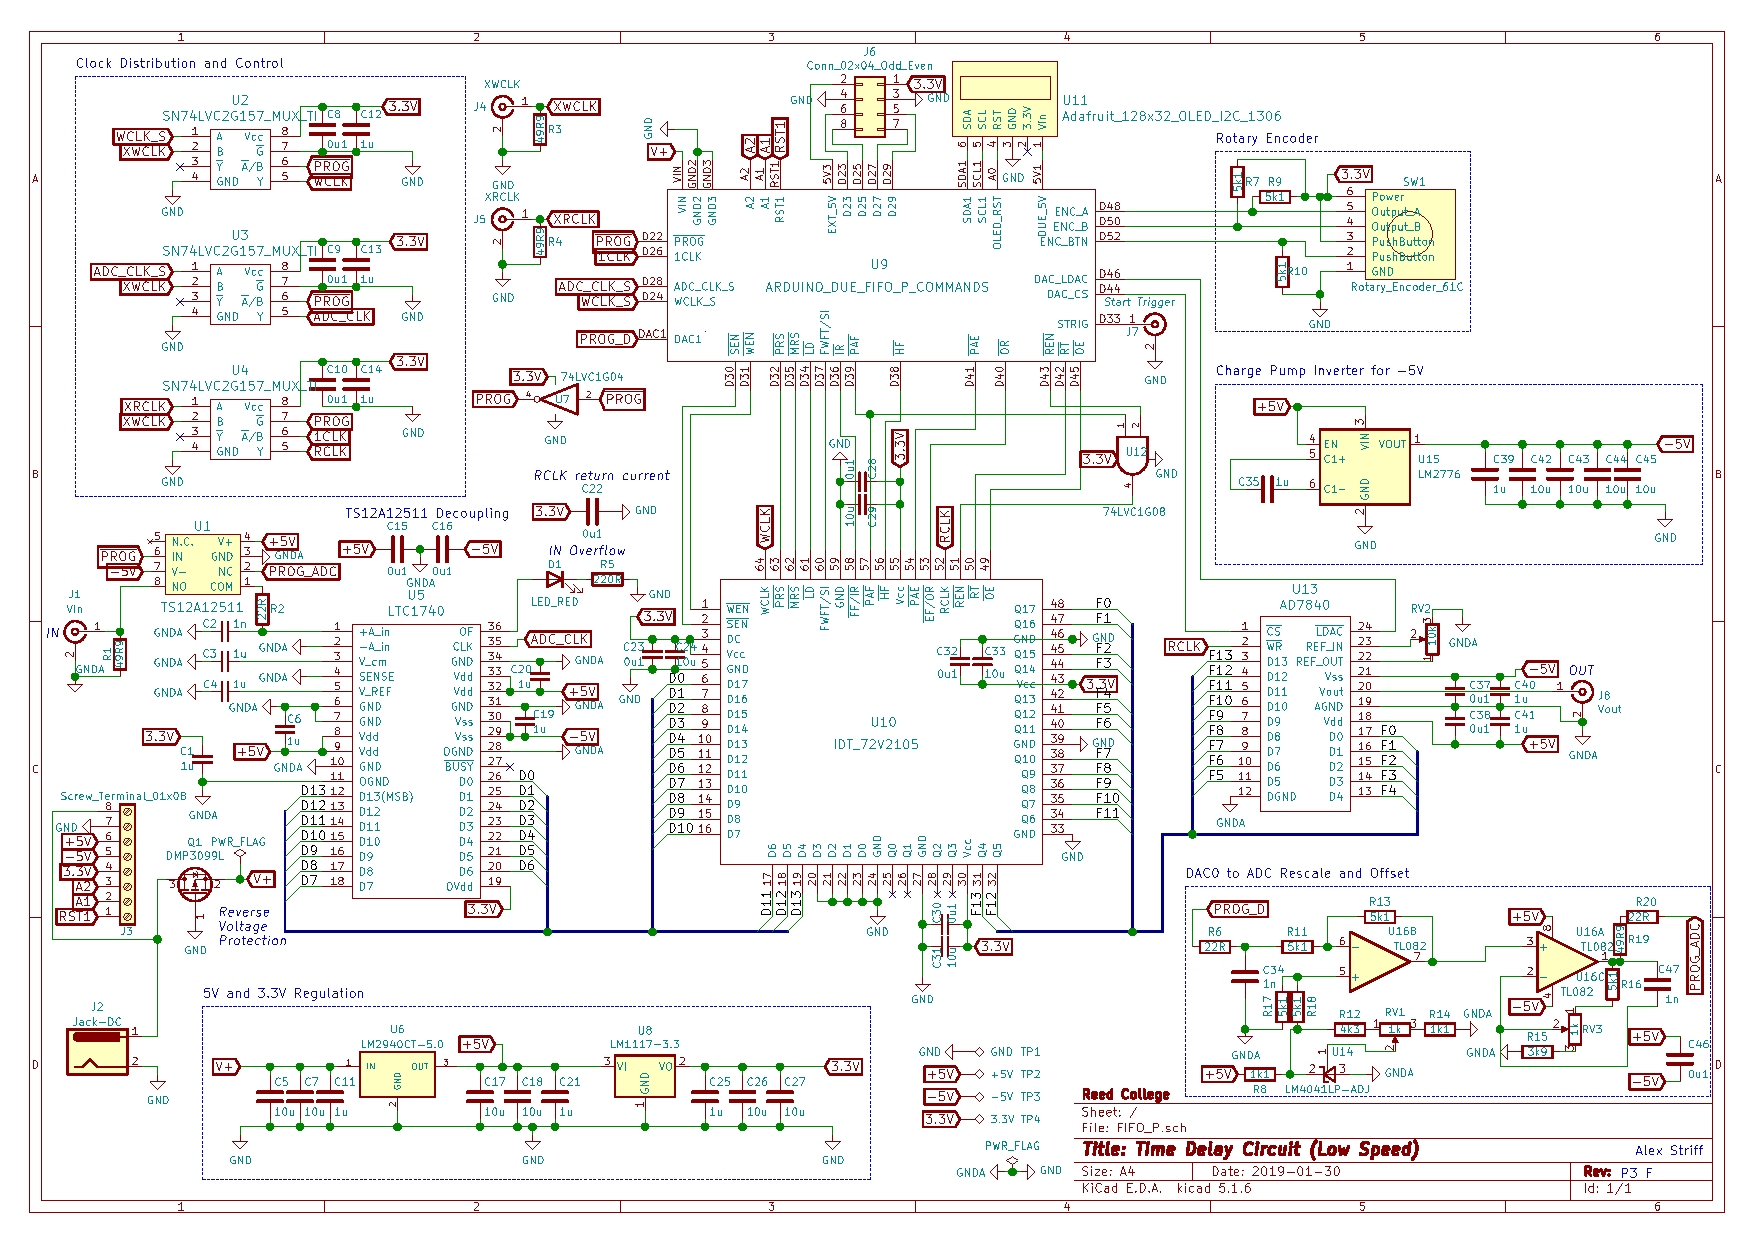
\includepdf[landscape]{../fifo-p3f/FIFO_P.pdf}
% \end{landscape}

\end{document}
